\begin{frame}[fragile]{Problema}

Em uma árvore binária, o percurso por nível é um percurso denominado \textit{breadth first search} (BFS) ou em português, busca em largura, a qual seria não-recursiva por natureza. Este percurso utiliza uma fila ao invés de pilha para armazenar os próximos 2 nodos que devem ser pesquisados (filho à esquerda e à direita). Esta é a razão pela qual você deve percorrer os nodos na ordem FIFO ao invés da ordem LIFO, obtendo desta forma a recursão.

Portanto nossa tarefa aqui, após algumas operações de inserção sobre uma árvore binária de busca (pesquisa), é imprimir o percurso por nível sobre estes nodos. Por exemplo, uma entrada com a sequência de valores inteiros: 8 3 10 14 6 4 13 7 1 resultará na seguinte árvore:

\end{frame}

\begin{frame}[fragile]{Problema}

    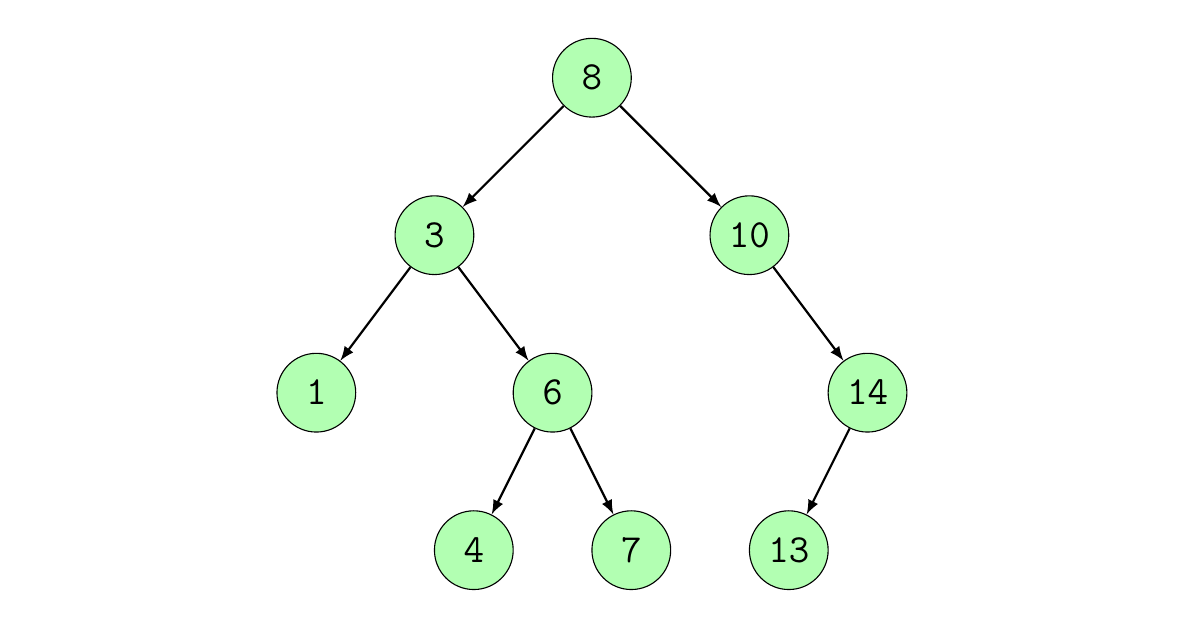
\begin{tikzpicture}
            \node[opacity=0] at (0, 7) { . };
            \node[opacity=0] at (14, 0) { . };

            \node[circle,draw,fill=green!30,minimum size=1cm] (A) at (7, 6.5) { \Large \tt 8 };
            \node[circle,draw,fill=green!30,minimum size=1cm] (B) at (5, 4.5) { \Large \tt 3 };
            \node[circle,draw,fill=green!30,minimum size=1cm] (C) at (9, 4.5) { \Large \tt 10 };
            \node[circle,draw,fill=green!30,minimum size=1cm] (D) at (3.5, 2.5) { \Large \tt 1 };
            \node[circle,draw,fill=green!30,minimum size=1cm] (E) at (6.5, 2.5) { \Large \tt 6 };
            \node[circle,draw,fill=green!30,minimum size=1cm] (F) at (10.5, 2.5) { \Large \tt 14 };
            \node[circle,draw,fill=green!30,minimum size=1cm] (G) at (5.5, 0.5) { \Large \tt 4 };
            \node[circle,draw,fill=green!30,minimum size=1cm] (H) at (7.5, 0.5) { \Large \tt 7 };
            \node[circle,draw,fill=green!30,minimum size=1cm] (I) at (9.5, 0.5) { \Large \tt 13 };

            \draw[-latex,thick] (A) to (B);
            \draw[-latex,thick] (A) to (C);
            \draw[-latex,thick] (B) to (D);
            \draw[-latex,thick] (B) to (E);
            \draw[-latex,thick] (C) to (F);
            \draw[-latex,thick] (E) to (G);
            \draw[-latex,thick] (E) to (H);
            \draw[-latex,thick] (F) to (I);
    \end{tikzpicture}

\end{frame}

\begin{frame}[fragile]{Entrada e saída}

\textbf{Entrada}

A entrada contém vários casos de teste. A primeira linha da entrada contém um inteiro $C$ $(C \leq 1000)$, indicando o número de casos de teste que virão a seguir. Cada caso de teste é composto por 2 linhas. A primeira linha contém um inteiro $N$ $(1 \leq N \leq 500)$ que indica a quantidade de números que deve compor cada árvore e a segunda linha contém $N$ inteiros distintos e não negativos, separados por um espaço em branco.

\end{frame}

\begin{frame}[fragile]{Entrada e saída}

\textbf{Saída}

Para cada caso de teste de entrada você deverá imprimir a mensagem \lq\lq Case $n$:", onde n indica o número do caso de teste seguido por uma linha contendo a listagem por nível dos nodos da árvore, conforme o exemplo abaixo. 

Obs: Não deve haver espaço em branco após o último item de cada linha e há uma linha em branco após cada caso de teste, inclusive após o último. A árvore resultante não terá nodos repetidos e também não terá mais do que 500 níveis.

\end{frame}


\begin{frame}[fragile]{Exemplo de entradas e saídas}

\begin{minipage}[t]{0.5\textwidth}
\textbf{Exemplo de Entrada}
\begin{verbatim}
2
3
5 2 7
9
8 3 10 14 6 4 13 7 1
\end{verbatim}
\end{minipage}
\begin{minipage}[t]{0.45\textwidth}
\textbf{Exemplo de Saída}
\begin{verbatim}
Case 1:
5 2 7

Case 2:
8 3 10 1 6 14 4 7 13
\end{verbatim}
\end{minipage}
\end{frame}

\begin{frame}[fragile]{Solução com complexidade $O(N^2)$}

    \begin{itemize}
        \item A solução deste problema é semelhante à do problema BEE 1195

        \item Novamente é necessário implementar o método construtor e a rotina de inserção 
            (a qual tem
            complexidade $O(S)$ no pior caso, onde $S$ é o tamanho da árvore)

        \item Além disso, é preciso implementar a travessia por largura (BFS)
            (cuja complexidade de cada travessia também é $O(S)$)

        \item Esta implementação é iterativa e requer o uso de uma fila para a organização do
            processamento dos nós

        \item Por fim, para cada caso de teste, basta instanciar uma árvore, inserir os elementos
            indicados e produzir a saída usando a travessia por largura
   \end{itemize}

\end{frame}

\begin{frame}[fragile]{Solução com complexidade $O(N^2)$}
    \inputsnippet{cpp}{1}{20}{codes/BEE1466.cpp}
\end{frame}

\begin{frame}[fragile]{Solução com complexidade $O(N^2)$}
    \inputsnippet{cpp}{22}{40}{codes/BEE1466.cpp}
\end{frame}

\begin{frame}[fragile]{Solução com complexidade $O(N^2)$}
    \inputsnippet{cpp}{42}{61}{codes/BEE1466.cpp}
\end{frame}

\begin{frame}[fragile]{Solução com complexidade $O(N^2)$}
    \inputsnippet{cpp}{63}{82}{codes/BEE1466.cpp}
\end{frame}
